%%%%%%%%%%%%%%%%%%%%%%%%%%%%%%%%%%%%%%%%%
% Masters/Doctoral Thesis 
% LaTeX Template
% Version 1.41 (9/9/13)
%
% This template has been downloaded from:
% http://www.latextemplates.com
%
% Original authors:
% Steven Gunn 
% http://users.ecs.soton.ac.uk/srg/softwaretools/document/templates/
% and
% Sunil Patel
% http://www.sunilpatel.co.uk/thesis-template/
%
% License:
% CC BY-NC-SA 3.0 (http://creativecommons.org/licenses/by-nc-sa/3.0/)
%
% Note:
% Make sure to edit document variables in the Thesis.cls file
%
%%%%%%%%%%%%%%%%%%%%%%%%%%%%%%%%%%%%%%%%%

%----------------------------------------------------------------------------------------
%	PACKAGES AND OTHER DOCUMENT CONFIGURATIONS
%----------------------------------------------------------------------------------------

\documentclass[11pt, a4paper, oneside]{Thesis} % Paper size, default font size and one-sided paper

\graphicspath{{Pictures/}} % Specifies the directory where pictures are stored

\usepackage{verbatim}
\usepackage[square, numbers, comma, sort&compress]{natbib} % Use the natbib reference package - read up on this to edit the reference style; if you want text (e.g. Smith et al., 2012) for the in-text references (instead of numbers), remove 'numbers' 
\usepackage{algorithm}
\usepackage{algorithmic}
\hypersetup{urlcolor=blue, colorlinks=true} % Colors hyperlinks in blue - change to black if annoying
\title{\ttitle} % Defines the thesis title - don't touch this

\begin{document}

\frontmatter % Use roman page numbering style (i, ii, iii, iv...) for the pre-content pages

\setstretch{1.3} % Line spacing of 1.3

% Define the page headers using the FancyHdr package and set up for one-sided printing
\fancyhead{} % Clears all page headers and footers
\rhead{\thepage} % Sets the right side header to show the page number
\lhead{} % Clears the left side page header

\pagestyle{fancy} % Finally, use the "fancy" page style to implement the FancyHdr headers

\newcommand{\HRule}{\rule{\linewidth}{0.5mm}} % New command to make the lines in the title page

% PDF meta-data
\hypersetup{pdftitle={\ttitle}}
\hypersetup{pdfsubject=\subjectname}
\hypersetup{pdfauthor=\authornames}
\hypersetup{pdfkeywords=\keywordnames}

%----------------------------------------------------------------------------------------
%	TITLE PAGE
%----------------------------------------------------------------------------------------

\begin{titlepage}
\begin{center}

\textsc{\LARGE Imperial College of London}\\[1.5cm] % University name
\textsc{\Large Research Project Report}\\[0.5cm] % Thesis type

\HRule \\[0.4cm] % Horizontal line
{\huge \bfseries Learning walking skills for Modular Robots}\\[0.4cm] % Thesis title
\HRule \\[1.5cm] % Horizontal line
 
\begin{minipage}{0.4\textwidth}
\begin{flushleft} \large
\emph{Author:}\\
Clement Jambou% Author name - remove the \href bracket to remove the link
\end{flushleft}
\end{minipage}
\begin{minipage}{0.4\textwidth}
\begin{flushright} \large
\emph{Supervisor:} \\
\supname % Supervisor name - remove the \href bracket to remove the link  
\end{flushright}
\end{minipage}\\[3cm]
 
%\large \textit{A thesis submitted in fulfilment of the requirements\\ for the degree of \degreename}\\[0.3cm] % University requirement text
%\textit{in the}\\[0.4cm]
%\groupname\\\deptname\\[2cm] % Research group name and department name
 


\includegraphics[scale=0.4]{Figures/Logo} % University/department logo - uncomment to place it


{\large \today}\\[4cm] % Date 
\vfill
\end{center}

\end{titlepage}
\clearpage
%----------------------------------------------------------------------------------------
%	DECLARATION PAGE
%	Your institution may give you a different text to place here
%----------------------------------------------------------------------------------------
\begin{comment}
\Declaration{

\addtocontents{toc}{\vspace{1em}} % Add a gap in the Contents, for aesthetics

I, \authornames, declare that this thesis titled, '\ttitle' and the work presented in it are my own. I confirm that:

\begin{itemize} 
\item[\tiny{$\blacksquare$}] This work was done wholly or mainly while in candidature for a research degree at this University.
\item[\tiny{$\blacksquare$}] Where any part of this thesis has previously been submitted for a degree or any other qualification at this University or any other institution, this has been clearly stated.
\item[\tiny{$\blacksquare$}] Where I have consulted the published work of others, this is always clearly attributed.
\item[\tiny{$\blacksquare$}] Where I have quoted from the work of others, the source is always given. With the exception of such quotations, this thesis is entirely my own work.
\item[\tiny{$\blacksquare$}] I have acknowledged all main sources of help.
\item[\tiny{$\blacksquare$}] Where the thesis is based on work done by myself jointly with others, I have made clear exactly what was done by others and what I have contributed myself.\\
\end{itemize}
 
Signed:\\
\rule[1em]{25em}{0.5pt} % This prints a line for the signature
 
Date:\\
\rule[1em]{25em}{0.5pt} % This prints a line to write the date
}

\clearpage % Start a new page
\end{comment}
\clearpage % Start a new page

%----------------------------------------------------------------------------------------
%	ABSTRACT PAGE
%----------------------------------------------------------------------------------------

\addtotoc{Abstract} % Add the "Abstract" page entry to the Contents

\abstract{\addtocontents{toc}{\vspace{1em}} % Add a gap in the Contents, for aesthetics
    
   In their design Modular Robots present many advantages when facing a task in a difficult environment. Among these advantages the way they could potentially adapt to this environment and reconfigure themselves when facing different tasks makes them the favorite candidate for many applications, such as space exploration. However controlling the swarm of robots from high-level commands remains a tricky problem, especially since this problem is non-linear and contains many degrees of freedom. Therefore it is resistant to classical approaches used in automation when dealing with Robotics motion control.


   The goal of this project is to present a survey of different control models and learning algorithms that proved to be efficient on similar problems. To compare these methods, we introduce a benchmark simulation built on the ODE Simulator and publicly available on Github. In this project we also apply for the first time Liquid State Machines to this particular problem of modular Robot locomotion. 
}

\clearpage % Start a new page

%----------------------------------------------------------------------------------------
%	ACKNOWLEDGEMENTS
%----------------------------------------------------------------------------------------

\setstretch{1.5} % Reset the line-spacing to 1.3 for body text (if it has changed)

\acknowledgements{\addtocontents{toc}{\vspace{1em}} % Add a gap in the Contents, for aesthetics

Professor Murray Shanahan, Department of Computing, Imperial College London

Professor Emmanuel Rachelson, Department of Mathematics, Computing and Automation, Supaero Graduate Program ISAE, Toulouse

Professor Jean-Marc Alliot, Department of Optimization and High Performance Computing, INRIT, Toulouse, Supaero Graduate Program, ISAE, Toulouse
%The acknowledgements and the people to thank go here, don't forget to include your project advisor\ldots
}
\clearpage % Start a new page

%----------------------------------------------------------------------------------------
%	LIST OF CONTENTS/FIGURES/TABLES PAGES
%----------------------------------------------------------------------------------------

\pagestyle{fancy} % The page style headers have been "empty" all this time, now use the "fancy" headers as defined before to bring them back

\lhead{\emph{Contents}} % Set the left side page header to "Contents"
\tableofcontents % Write out the Table of Contents

\lhead{\emph{List of Figures}} % Set the left side page header to "List of Figures"
\listoffigures % Write out the List of Figures

%\lhead{\emph{List of Tables}} % Set the left side page header to "List of Tables"
%\listoftables % Write out the List of Tables

%----------------------------------------------------------------------------------------
%	ABBREVIATIONS
%----------------------------------------------------------------------------------------
\begin{comment}
\clearpage % Start a new page

\setstretch{1.5} % Set the line spacing to 1.5, this makes the following tables easier to read

\lhead{\emph{Abbreviations}} % Set the left side page header to "Abbreviations"
\listofsymbols{ll} % Include a list of Abbreviations (a table of two columns)
{
\textbf{LAH} & \textbf{L}ist \textbf{A}bbreviations \textbf{H}ere \\
%\textbf{Acronym} & \textbf{W}hat (it) \textbf{S}tands \textbf{F}or \\
}

%----------------------------------------------------------------------------------------
%	PHYSICAL CONSTANTS/OTHER DEFINITIONS
%----------------------------------------------------------------------------------------

\clearpage % Start a new page

\lhead{\emph{Physical Constants}} % Set the left side page header to "Physical Constants"

\listofconstants{lrcl} % Include a list of Physical Constants (a four column table)
{
Speed of Light & $c$ & $=$ & $2.997\ 924\ 58\times10^{8}\ \mbox{ms}^{-\mbox{s}}$ (exact)\\
% Constant Name & Symbol & = & Constant Value (with units) \\
}

%----------------------------------------------------------------------------------------
%	SYMBOLS
%----------------------------------------------------------------------------------------

\clearpage % Start a new page

\lhead{\emph{Symbols}} % Set the left side page header to "Symbols"

\listofnomenclature{lll} % Include a list of Symbols (a three column table)
{
$a$ & distance & m \\
$P$ & power & W (Js$^{-1}$) \\
% Symbol & Name & Unit \\

& & \\ % Gap to separate the Roman symbols from the Greek

$\omega$ & angular frequency & rads$^{-1}$ \\
% Symbol & Name & Unit \\
}

%----------------------------------------------------------------------------------------
%	DEDICATION
%----------------------------------------------------------------------------------------

\setstretch{1.3} % Return the line spacing back to 1.3

\pagestyle{empty} % Page style needs to be empty for this page

\dedicatory{For/Dedicated to/To my\ldots} % Dedication text

\addtocontents{toc}{\vspace{2em}} % Add a gap in the Contents, for aesthetics

\end{comment}
%----------------------------------------------------------------------------------------
%	THESIS CONTENT - CHAPTERS
%----------------------------------------------------------------------------------------

\mainmatter % Begin numeric (1,2,3...) page numbering

\pagestyle{fancy} % Return the page headers back to the "fancy" style

% Include the chapters of the thesis as separate files from the Chapters folder
% Uncomment the lines as you write the chapters

% Chapter Template

\chapter{Related Work} % Main chapter title

\label{Chapter 1} % Change X to a consecutive number; for referencing this chapter elsewhere, use \ref{ChapterX}

\lhead{Chapter 1. \emph{Related Work}} % Change X to a consecutive number; this is for the header on each page - perhaps a shortened title

%----------------------------------------------------------------------------------------
%	SECTION 1
%----------------------------------------------------------------------------------------

%\section{State of the Art}

\section{Overview}
For over two decades, motion learning for complex structure has been a research focus. There has been many different approach to this problem, but it usually involves a simulated environment, where the creature can experiment with and get feedback from. The general problem is for this creature to learn by itself how to move in this environment in order to maximize a certain quantity such as its speed or distance with a certain amount of energy. The creature can have different ways of controlling its body using actuators to control the angle of its joints, (or even simulated muscles) and eventually some sensors to get feedback from the world. The goal being to generate the control function  $\alpha_i(t, state) $ for each actuator's degree of freedom, that link time $t$ and eventually the state of the creature to a command that can be send to the actuator (an angle for a servomotor, or command to a motor, an electrical signal to a simulated muscle ...). A widely used approach so far, which makes sense from a biological perspective is to implement smart actuators that can be linked directly to a sensor and modify the command with a low-level control. One of the examples of this behaviour is the muscle elasticity, which will alter the consequence of a specific command depending on the state of the muscle. Another example is the Proportional-Integral-Derivative controller (PID) of a servomotor. It is then possible to build a model that behaves as an open-loop from a high level perspective, but which actually shows robustness due to this low-level control loops. 
Under this assumption, we have the function $\alpha_i(t)$ that are only depending on parameter $t$. Finding the set of these functions remains an optimization problem in an infinite dimensional space. Therefore it is useful to make another assumption, which is that these functions are periodic. This make sense when we observe the movements of animals in the nature. In fact we can even consider the paradigm of oscillation based movements in the nature and apply it to the $\alpha_i(t)$ functions and write them using Fourier decomposition. $$\alpha_i(t) = \sum_{k = 1}^N {b_{ki} * sin(kt)} + \sum_{k = 1}^N {b_{-ki} *  cos(kt)} + b_{0i} $$.
With this decomposition, we transform our infinite dimensional research space ( of functions ) to a finite one containing the $b_{ki}$ ($ -N <= k <= N $) coefficients. The parameter $N$ is a restriction over the harmonics and can be seen as a precision parameter that determines how near we can get from any periodic function. This space of research remains big and does not reflects in its structure any of the physical interaction that can exist between two actuators (symmetry, graph structure) of the creature. Therefore, some of the following related works use different techniques to reduce the dimension of the space and also different learning techniques to obtain a solution. 

\section{Karl Sims Creatures}
The first remarquable examples of modular robotics learning to evolve in a 3D simulated world is due to Karl Sims's Creature in 1994 \cite{karl}. In his work, the structure of the creature evolves at the same time as the control system. One way of reducing the search space of Fourier coefficients is to create a graph that generate oscillation (much like the brain of animals does). The neural network used in Karl's creature takes as input a set of values from different sensors and each node can perform a specific function such as sums, products, a logical functions, and trigonometric functions to generate the oscillations of the structure. He also uses Genetic Algorithms in order to optimize all the parameters of the control graph and the structure. See the Chapter of Learning Methods for a detail explanation on Genetic Algorithms. 

\section{Central Pattern Generators}
Other techniques using Central Pattern Generators (CPG) have been used on modular structures at EPFL \cite{marbach} \cite{sproewitz}. The CPG is a graph that relates directly to the physical structure in order to generate oscillation. So it is also a technique to reduce the dimension of Fourier coefficients space to simplify the problem and reflect the physical structure of the creature using coupled oscillators. \cite{marbach} used another type of optimization techniques to do online learning of a subset of the parameters and find a local minima.

More recently, the progress of computational power and the growing interest of building humanoid robots for different tasks in non-friendly environment, such as the initiative from Virginia Tech to build a disaster response robots, or the growing demand of the animation movie and video games industry led to new results. The approach of \cite{MuscleBasedBipeds} uses muscle-based actuators and optimize at the same time the routing of the muscles and the control of the muscle activation from a musculoskeletal model. This approach showed robust locomotion for different speed, target directions and small ground variations in terrain.


% Chapter Template

\chapter{Simulation Environment} % Main chapter title

\label{Chapter 1} % Change X to a consecutive number; for referencing this chapter elsewhere, use \ref{ChapterX}

\lhead{Chapter 1. \emph{Simulation Environment}} % Change X to a consecutive number; this is for the header on each page - perhaps a shortened title

%----------------------------------------------------------------------------------------
%	SECTION 1
%----------------------------------------------------------------------------------------
The first task of my project was to build a simulator to be able to get feedback from a simulated world. The goal of the simulator is to provide an environment which is governed by physics laws. In this project such physics laws are gravity, friction and collisisons. Combining this two phenomena on complex structure can lead to situations difficult to predict, especially since it has a chaotic behavior. Two movements of a structure in such a physical world, though they differ just a little, can lead to very different outcomes.  

\section{Physics Engine}

In order to simulate the behavior of complex shapes and bodies in a simulated world, a physical engine is required. This kind of physical engine is used in a lot of different areas, for instance the film and video games industry, to simulate destructions or complex situations where placing all bodies by hand would be too difficult. I tested two different librairies that provide tools to simulate these complex situtations : \verb?bullet? \verb?ODE? (\verb?Open Dynamics Engine?). The first part was to simulate the static part of the world, which is the ground. For now, I used a plane, with a friction coefficient, but we can imagine testing all the structure on different surfaces, (not necessarly plans). Also in order to simplify the structure, so that the modules are simple shapes, all the robots are only composed of cubes, linked by different type of joints. ODE and bullet also provide tools to simulate joints (adding constraint on the relative movements of different bodies) and also to animate them simulating motors. I choose ODE for its simplicity to control different joints using this motors. In order to simulate a servomotor properly, it is for instance possible to set a maximimum torque value and a command to the motor.

\begin{figure}[htbp]
    \centering
    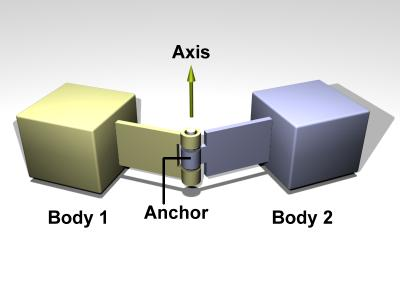
\includegraphics{Figures/hinge.jpg}
    \rule{35em}{0.5pt}
    \caption[A Hinge Constraint]{A 3D representation of a Hinge Constrain}
    \label{fig:Hinge}
\end{figure}

\section{Visual rendering}
A good thing about the physical engine is that it is completly separated from the rendering part. That way, it is possible to run much faster for the learning process. But it is also necessary to see the result, especially for the purpose of debuging the simulator. Carnegie Mellon University developps a framework called panda3d, that integrate both a rendering librairy using OpenGl and different physics engines (ODE and bullet). All this tools are developped in C/C++ with binding for python, which makes it an easy tool to create animation movie, games or simulations.


\begin{figure}[htbp]
    \centering
    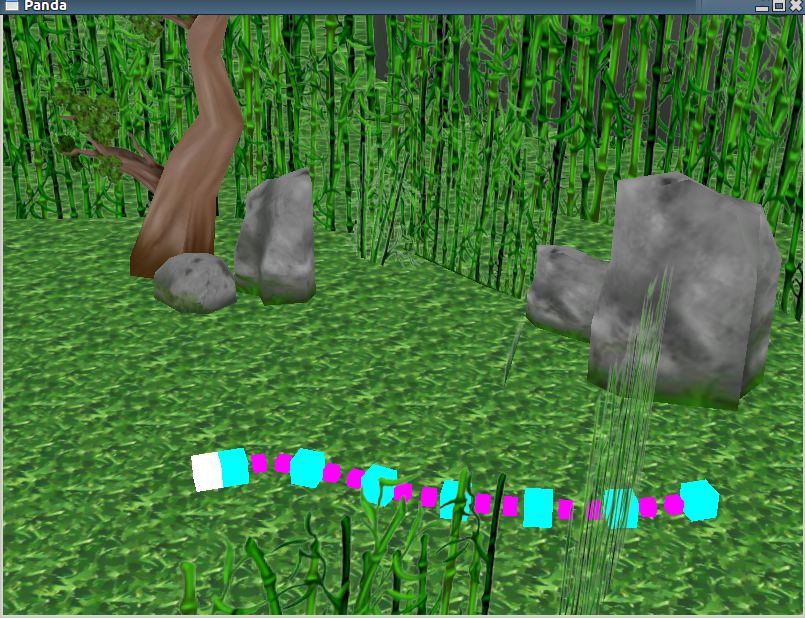
\includegraphics[scale=0.5]{Figures/snake.png}
    \rule{35em}{0.5pt}
    \caption[Simulated Snake in the environment]{3D Rendering of a snake in the environment}
    \label{fig:Snake}
\end{figure}



\subsection{The coordinate system}
In order to represent all the objects that we manipulate in the simulation (physics and rendering), panda3d uses a system of global/local coordinate and a tree architecture. Each element of the tree is represented in the coordinates of the father. In order to keep a coherence with this architecture, it is natural to use a graph to represent the modular structure of the robots. Panda3d also uses 4-by-4 matrices to represent the transformation of a node to its one of its children. These transformation are classical in 3d representation. They combine the benefits of 3 by 3 matrices that represent functions ($\mathbb{R}^3 \to \mathbb{R}^3$) that can be interpreted as the set of combined rotations and homotetia, where the matrix multiplication is the composition of such transformations, and a translation. Manipulating translations requires to use 4 by 4 matrices instead of 3 by 3 but the properties of the product are kept, which makes it a very useful tool to manipulate 3d objects. For instance, if the children of the node is translated of a vector $(1, 0, 0)$, then we can use a function on the object representing the Matrice (TransformState in panda3d) to change the matrice and add the translation. The same goes for giving a certain orientation to the object using quaternions to represent the 3D orientation and add this to the 4 by 4 matrix.

## Picture of the 4*4 Matrix ##

\section{Structures of the Robots as a Graph} 

We can represent a Robot as a graph, where each node is a component of the robot. In this project there is four types of components : 
\begin{itemize}
    \item the head: which has a cube shapes and 6 sons (one for each faces), There is only one head per structure.
    \item a structural block: This is also a cube, also with 6 sons (or edges in the graph) for all faces.
    \item a hinge joint: The hinge is composed of two small cubes, separated by the joint whith one degree of freedom.
    \item a vertebra : a vertebra is very much like a hinge but has two degrees of freedom (two angle directions) with smaller range, but bigger maximal torque.
\end{itemize}

## Picture of Hinge and vertebra ? ##

This Structure is represented in python with an object called MetaStructure, with very simple function to move within the graph and add components and follow edges that make it easy to design a structure that we have in mind, ( or for possible later use to generate them automaticly\ldots). This object is the key to describe a structure.  


\begin{figure}[htbp]
    \centering
    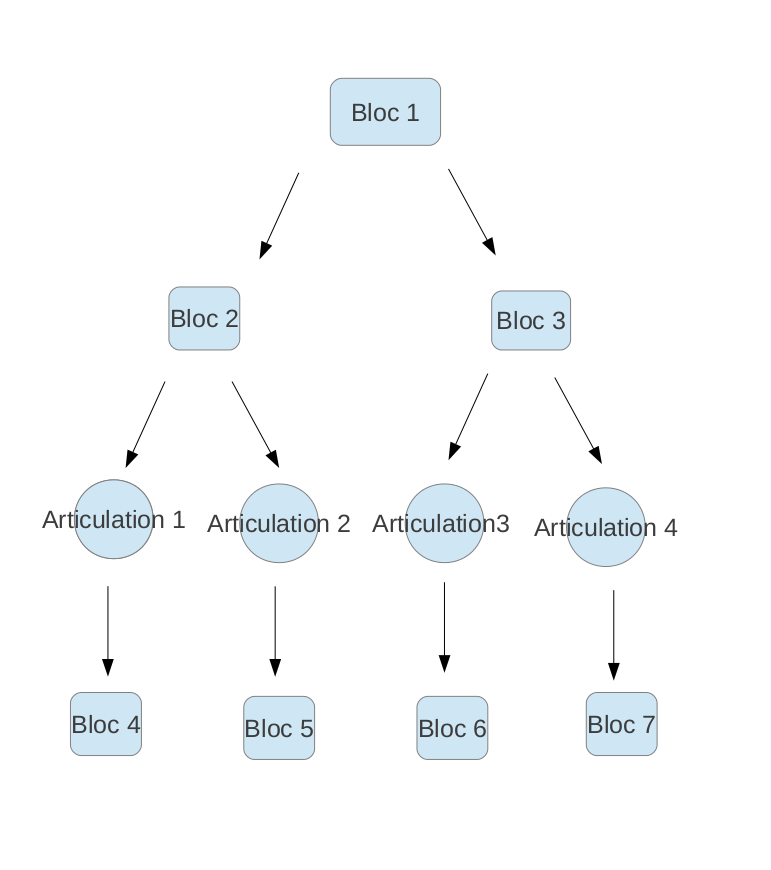
\includegraphics[scale=0.5]{Figures/schema_arbre.png}
    \rule{35em}{0.5pt}
    \caption[Structure described as graph]{Structure described as a graph}
    \label{fig:Snake}
\end{figure}



% Chapter Template

\chapter{Control} % Main chapter title

\label{Chapter 3} % Change X to a consecutive number; for referencing this chapter elsewhere, use \ref{ChapterX}

\lhead{Chapter 3. \emph{Control}} % Change X to a consecutive number; this is for the header on each page - perhaps a shortened title

%
Once the simulation is fully implemented, the goal is to use it as a testbench for different ways of controlling the structure. The second part of the project was fully consecrated on this part. PID (Proportionnal-Integrate-Derivative) control loops have been implemented to make sure that the command is respected by the creatures. Three different model were implemented and tested to control the creature: Fourier Decomposition, Central Pattern Generators and Liquid State Machines. The goal of each of these models is to represent the $\alpha_i(t)$ functions that are the angle of the joints with a vector of finite size. The Fourier Decomposition model for example (see Introduction) represent the angle functions with their Fourier Decomposition.

\begin{figure}[htbp]
    \centering
    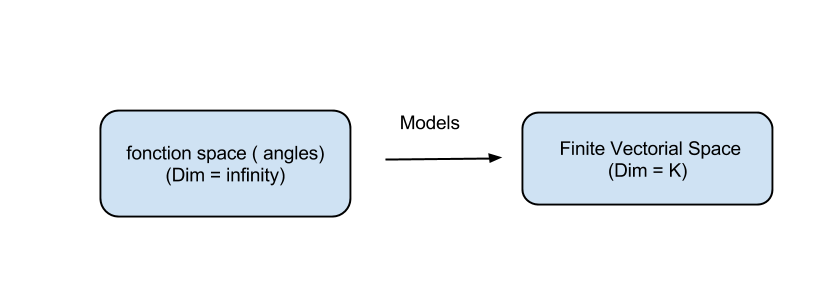
\includegraphics[scale=0.5]{Figures/models.png}
    \rule{35em}{0.5pt}
    \caption[Learning Model]{Learning Model}
    \label{fig:models}
\end{figure}

The two other models are described in this chapter.

\section{PID Control of the joints}

One of the problem to control accurately a joint is to adapt the command so that it can adapt to difficult situation. For instance, it is easier to walk in a swimmingpool than on the ground and this is why people recovering after an injury do aquatic training. For a joint, it can be easy to do a movement in the air, but the same movement is more difficult when touching the ground. One way to avoid this problem is to implement PID (Proportional Integral Derivative) controller. This kind of controller is used in a lot of different situation in the world of automation to control degrees of freedom. In or case, servomotors often integrate such loops to account for these changes of use. In the simulation, at each step, the command of each degree of freedom of the structure is calculated using such a PID controller. 

\begin{figure}[htbp]
    \centering
    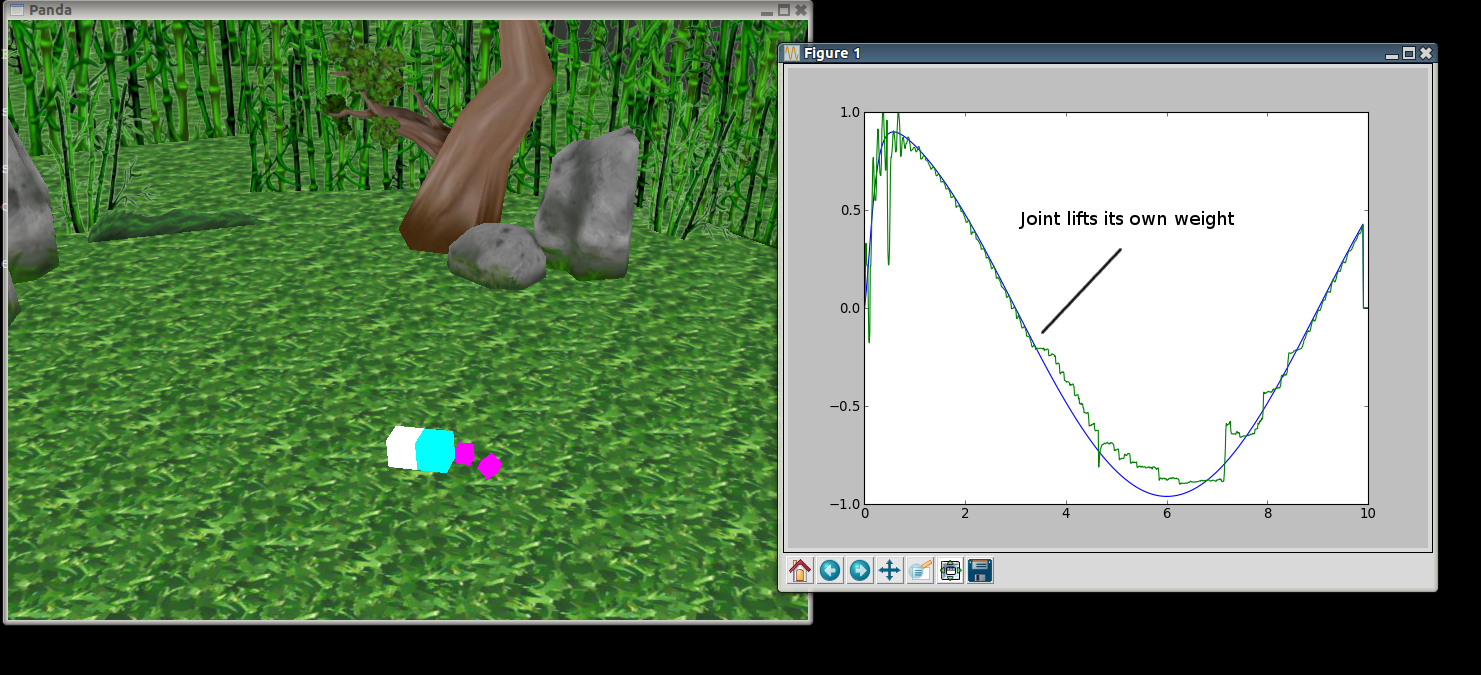
\includegraphics[scale=0.3]{Figures/servomotor.png}
    \rule{35em}{0.5pt}
    \caption[Answer of a joint to a sinusoid command]{Answer of the joint to a sinusoid command with PID Control}
    \label{fig:Snake}
\end{figure}

One of the problem with the control of the joints is the unstability. On the simulation, as the angles have periodic values, if the joint has a high angle velocity, then between two steps, it can jump accross the boundary and start turning faster and faster as the PID controller will not be able to work as well as if the degree of freedom were a linear parpameter. The problem with this situation is that it can actually be seen as a good result for the learning algorithm, simply because the fitness function is the velocity of the creature. There are several things to prevent from this situation :

\begin{itemize}
    \item reduce the time between two steps of computation for the physics engine and the PID
    \item reduce the maximum torque available per joint
    \item punish the creature if the joints are moving to slow
    \item change the fitness function to maximize parameter under a certain energy level
\end{itemize}
        

Another issue is more a biological concern. The main goal of this project is to find solutions that are biologically inspired instead of using a classical automation approach (eventhough we can compare the elasticity of or muscles as such controllers\ldots). Therefore though the use of PID is necessary in many robotics applications, we will try to avoid using the in the second part of the project. 

\section{Central Pattern Generator}

Central Pattern Generators (CPGs) are neural networks, that can generate oscillation for the control of the muscles of or body. They are the consequence and the cause of the paradigm of periodic movement in the locomation of animals. Different models have been implemented to represent CPGs. We can represent them as a graph of coupled oscillator, where each node influence the behavior of its neighbours. For a first implementation I choose to test the model of CPG followed at EPFL (\cite{sproewitz}). 

The CPG Neural Network in that case, is a graph that follow the physical architecture of the robot, settting one node for each joint (hinge or vertebra) on the structure. The dynamic of the CPG is determined by a coupling weight matrix $w_{ij}$, a phase bias matrix between nodes $\varphi_{ij}$, the frequency of the different oscillator $\omega_i$ and the desired amplitude and offset of the oscillation. We can compute the angle using the following system of equation and an integration method (I used the Runge-Kutta method in this project)

\begin{equation*}
    \dot{\phi_i} = \omega_i + \sum{w_{ij} * r_j * sin(\phi_i - \phi_j - \varphi_{ij})} \tag{1}
\end{equation*}
\begin{equation*}
        \theta_i = x_i + r_i * cos(\phi_i)  \tag{2}
\end{equation*}
This two equation gives the angle of the oscillator ($\theta_i$) depending on the state variable of a node: $x_i$, $r_i$, $\phi_i$, that can be described respectively as the offset, the amplitude and the phase of the oscillator.

\begin{equation*}
    \acute{r_i} = ar(\frac ar (R_i - r_i) - \dot{r_i}) \tag{3}
\end{equation*}
\begin{equation*}
    \acute{x_i} = ax(\frac ax (X_i - x_i) - \dot{x_i}) \tag{4}
\end{equation*}

Equations (3) and (4) describe the dynamic of the amplitude and offset (a second order dynamic that converge to the desired values). This trick is to ensure continuity in the oscillations, even if some of the parameters of the oscillator change. $a_r$ and $a_x$ are gains to control the dynamic ($a_r = a_x = 20 rad/s$  \cite{sproewitz}). 


A modification of this model is possible to plug the measured value of the degrees of freedom. Instead of using the second order control loop on $\theta_i$ which is achieved with the PID, we can set this control on the phase. Thatway, if the joint has troubles achieving his movement, for instance when hitting the ground, the phase will be modified and the perturbation will have an impact on othe joints through equation (1).

Oneway to do so is to add a term in the equation (1), with $\dot{\theta_{reali}}$ the mesured angle velocity of the joint. 
\begin{equation*}
    \dot{\phi_i} = \omega_i + \sum{w_{ij} * r_j * sin(\phi_i - \phi_j - \varphi_{ij}) + a_{\phi} * \frac {\dot{\theta_{reali}} - \dot{\theta_i}} {r_i * sin (\phi_i)}} \tag{1}
\end{equation*}

If we derive (2) we get: 
\begin{equation*}
    \dot{\theta_i} = \dot{x_i} + \dot{r_i} * cos(\phi_i) + r_i * sin(\phi_i) * \dot{\phi_i} \tag{2'}
\end{equation*}

By making the assumption that the dynamic of the amplitude and the offset is slow compared to the phase, we get
\begin{equation*}
    \dot{\theta_i} = r_i * sin(\phi_i) * \dot{\phi_i} \tag{2''}
\end{equation*}
Thatway, if we consider small variation of the phase, we can deduce an error term on $\dot{\phi_i}$ from the error on $\dot{\theta_i}$ given by $\frac {\dot{\theta_{reali}} - \dot{\theta_i}} {r_i * sin (\phi_i)}$ that we can control with a gain ($a_{\phi}$).
For example if the movement of a joint is made difficult because of the ground, then the mesured velocity of this joint will be smaller that expected. The consequence will be to accelerate the movement for this joint (the derivative of the phase will be bigger), but also for the other joints that are linked to this one. We can interprete this as neural communication in our body within the central pattern generator, but also as the elasticity between joints. For instance if achieving a movement is too difficult for a joint, using elasticity, it is possible to get help from joints that are near. 


\section{Liquid State Machine}

Liquid State Machine (LSM) and Echo State Network were independantly and simultaneously introduced by Mass and al \cite{liquidstatemachine} and Jaeger and al. \cite{echostatejaeger} and present a way of generating oscillations \cite{echostate}. They were introduced as a way of using recurrent neural network for Machine learning purposes, as recurrent neural network are harder to train using the classical backpropagation algorithm. A LSM is created from a random recurrent neural network that contains N neurons and is called the reservoir. The state of the neurons in the reservoir are updated using the following equation: 
\begin{equation*}
    X_{t + 1} = f( W_r * X_{t})
\end{equation*}
 where $W_r$ is the random weight matrix inside the reservoir and f is the activation fonction ( in this project we used the hyperbolic tangent as the activation function)

Once this network is created, oscillations can be observed in the state of each neurons. A weight matrix is randomly initiated to produce linear combinations of these oscillations that can be plugged to control the joints angles of the creature.

\begin{equation*}
    \alpha_i(t) = \frac{\pi}{2} f( W_o * X_{t})
\end{equation*}

where $W_o$ is the output weights and f is also an activation function. We then multiply the results by $\frac{\pi}{2}$ to ensure that the angles are in an acceptable range for the control in any situation.

\begin{figure}[htbp]
    \centering
    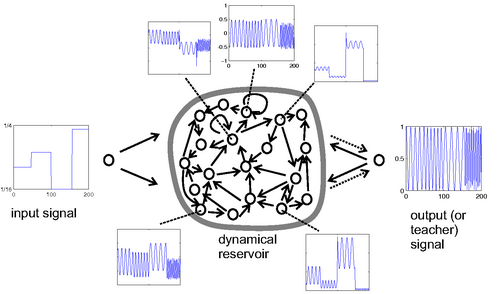
\includegraphics[scale=3.0]{Figures/echo_state.png}
    \rule{35em}{0.5pt}
    \caption[Liquid State Machine]{Liquid State Machine}
    \label{fig:echo_state}
\end{figure}


The idea of the Liquid State Machine is to focus the learning parameters on the output weights. The reservoir of neurons can be big, and produce a large variety of periodic signals. By learning the $W_o$ matrix ( of size $N * K$ where $N$ is the size of the reservoir and $K$ the number of hinge) each hinge can select some features of these oscillations. 

It is also possible to use a feedback loop in the network, by plugging the mesured angles in the reservoir using the output weights. 

 



 
% Chapter Template

\chapter{Learning Methods} % Main chapter title

\label{Chapter 4} % Change X to a consecutive number; for referencing this chapter elsewhere, use \ref{ChapterX}

\lhead{Chapter 4. \emph{Learning Methods}} % Change X to a consecutive number; this is for the header on each page - perhaps a shortened title

In this chapter we present different Learning Methods that have been tested and compared on this particular problem. All of these methods are optimization algorithms to find a minimum (or a maximum) over a set of parameters. It is not possible to get a gradient or Hessian matrix for a problem involving a simulation as fitness function. Therefore none of these algorithms use the derivatives of the function as information to find optima (unlike Gradient Method or Broyden-Fletcher-Goldfarb-Shanno (BFGS)). The following sections present different algorithms that can perform such a task. We then compare their results on the simulation. For coherence in this chapter, we use the following notation: 

\begin{itemize}
    \item $X = \{ X_p, p\in{\{1, ..., q\}}\} $ is a set of $q$ elements (or vectors) of the parameter space ($\mathbf{R}^ n $), where $n$ is the dimension of this space. $X_{p,i}$ is a scalar, and represent the $i$-th coordinate of the $p$-th element of the population.
    \item $f (\mathbf{R} ^ n \to \mathbf{R})$ is the fitness function we want to minimize.
    \item $X^{(p)}$ the p first element of the ordered list of element from set $X$ where the order relation is given by $X_i \leq X_j$ iff $f(X_i) \leq f(X_j)$
    \item iterators $p, q$ are over the population, where $i, j$ are over the coordinate of each element  
\end{itemize}

\section{Genetic Algorithm}

A Genetic Algorithm (GA) is an optimization algorithm that replicate the process of natural evolution. GAs were introduced in the 60s and early 70s and are inspired from biology. They consist of a loop of four steps until convergence (or a proper solution) is reached : evaluation, selection, cross-over, mutation. A population $X$ of $p$ elements is randomly generated to initialize the algorithm. The evaluation step is just running the fitness function $f$ over the new elements.

\subsection{Selection} 
The first step is a selection step. The goal is to keep only a part of the population and eliminate the rest. This is directly related to Natural Selection, where the "weekest " animals are less likely to survive. They are different ways of keeping "good elements". The first idea that comes to mind in performing such a step is to keep the $q$ best elements, ie $X^{(q)}$. The problem with this solution is that it prevent the population from "exploring" as all the best elements will be kept, it is more likely for the population to get stuck into a local minima. A widely use alternative is the Tournament Selection. We randomly select two elements and keep only the best of the two. We repeat this step until enough elements have been eliminated (usually half of the population). This alternative give a chance to all elements even if they are not in $X^\{q}$ best.  

\begin{algorithm}
    \caption{Tournament Selection}
    \begin{algorithmic}
    \STATE $ p = 0 $
        \WHILE{$p < q / 2$}
            \STATE $ X_1 = random element(X) $ 
            \STATE $ X_2 = random element(X) $
            \IF{$f(X_1 \leq X_2)$}
                \STATE $X.eliminate(X_2)$
            \ELSE
                \STATE $X.eliminate(X_1)$
            \ENDIF
        \ENDWHILE
    
    \end{algorithmic}
\end{algorithm}

\subsection{Cross-Over}
    The cross-over is a step to repopulate after the selection. By taking two random elements of the set, we can compute new elements (usually 2) by performing a cross-over of the the two parents. This step is inspired from reproduction in biology. The idea behind it is that by taking two good solutions, we can create 2 new elements that are likely to be good solutions. When the elements are scalar, a way of producing these solution is to use a barycenter of two solutions. 

\begin{algorithm}
    \caption{Cross-Over}

    \begin{algorithmic}
    \FOR{$p \in [1: q/2]$}
            \STATE $X_1 = random element(X)$
            \STATE $X_2 = random element(X)$
            \STATE $\lambda = random float([0.5; 1.5])$
            \STATE $X.add (\lambda * X_1 + ( 1 - \lambda) * X_2)$
            \STATE $X.add (\lambda * X_2 + ( 1 - \lambda) * X_1)$
    \ENDFOR
    \end{algorithmic}
\end{algorithm}


\subsection{Mutation}
    Finally the mutation step is a way of exploring new solutions. We randomly chose some elements to be mutated and modify them slightly. One way of doing the mutation when dealing with vector of real numbers is to use a gaussian distribution which use the previous elements as a mean, and a covariance matrix that depends of the population (for instance the covariance of p-nearest neighbors)

\subsection{Discussion on the hyper parameters}


\section{Nelder-Mead method}

The Nelder Mead method (or downhill simplex method) is a way of finding a local optimum, without knowing the gradient of the function in a given multidimensional space. We initialize a non-degenerated simplex in this space, then we follow this procedure (source: wikipedia):
\begin{itemize}
    \item Ordering: we order the points of the simplex such that $f(x_0) >= f(x_1) >= f(x_2) \dot >= f(x_n)$, where f is the fitness function that we want to maximize ( traveled distance...)
    \item We compute the center of gravity of all the points $x_g$

    \item We compute the reflection of $x_n$ in respect to $x_g$ ($x_r = x_g + (x_g - x_n )$)

    \item If $f(x_r) > f(x_{n - 1})$ then we compute the expansion point : $x_e = x_g + 2 * (x_g - x_n )$ if $f(x_e) > f(x_r)$ we replace $x_n$ with $x_e$ else $x_r$ and we go back to the first step.

    \item If $f(x_r) > f(x_{n - 1})$ then we compute the contraction point : $x_c = x_g + 0.5 * (x_g - x_n )$ if $f(x_c) > f(x_n)$ we replace $x_n$ with $x_c$ and go back to the first step, else we do the next step

    \item a contraction homotethia of center $x_0$ : we replace $x_i$ with : $x_i = x_0 + 0.5 * (x_i - x_0 )$ for $i > 0$ and go back to the first step.
\end{itemize}
 
\begin{figure}[htbp]
    \centering
    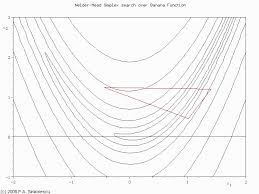
\includegraphics[scale=0.7]{Figures/nelder_mead.jpg}
    \rule{35em}{0.5pt}
    \caption[A simplex following the Nelder-Mead method]{A simplex following the Nelder-Mead method}
    \label{fig:nelder_mead}
\end{figure}



Moreover, in this problem the fitness function is not likely to be convex, as taking the mean of two good solutions for the movement of a structure does not necessary provide a good solution. The fitness function can also present some discontinuities or high variations because of collisions. Collisions are not continuous phenomena and even if the physics engine use smoothing techniques to simplify interractions. For instance there is a very small difference between a biped structure walking and a biped structure almost walking but with one leg that does not touch the ground, but the fitness function will give completely different results as one structure is moving and the other is not. Finally there is also the problem of consistency of a result, because two structures can behave differently for the same parameters, as the simulation can show chaotic behavior as small variations can have a big impact on the movement. For all these reasons, it is difficult to use classical optimisation for the creatures to learn how to move in the simulated environment. 





It is then possible to learn the parameters of the CPG to optimize the movement of the structure. Instead of having to find the value of the angles, the CPGs act as basis function for the angles, and thatway we reduce the space of research to a space with finite dimensions. All the parameters (frequency, offset and amplitude of each node) are scaled to fit between $0$ and $1$. A simple fitness function can be extracted from the simulation, for example the distance traveled by the head of the structure. 
\begin{figure}[htbp]
    \centering
    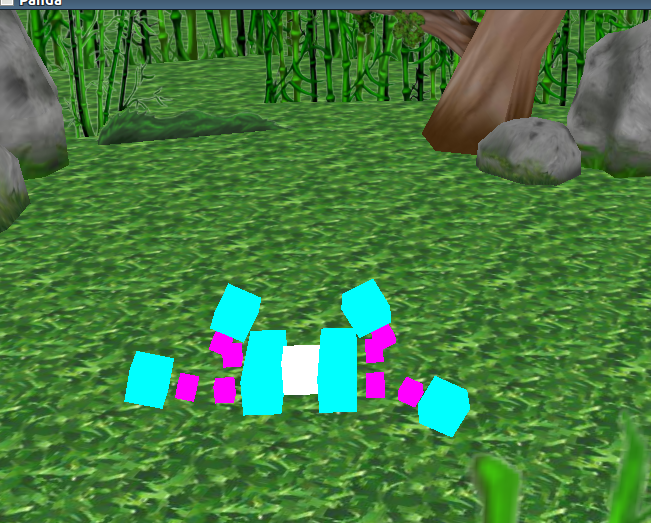
\includegraphics[scale=0.5]{Figures/four_legged.png}
    \rule{35em}{0.5pt}
    \caption[A structure with four legs learning]{A structure with four legs learning}
    \label{fig:four_legged}
\end{figure}

\section{Random Search}

A first very simple way of finding good solution is random search. We test a random set of parameters and keep the vector of parameters showing the best results. This has the benefit of being very simple to implement and provides a good testbench for fixing issues with the simulation. A first problem observed was the consistency of the solution, testing the same parameters can lead to very different results. A first way to correct this was to take longer sample (about 20 sec of simulation). Even with this correction, online learning brought some issues, as it is possible that a good results is only good because of the initial configuration given by testing previous movement. A way to correct this is to set all angles to a default value and wait for the structure to be have a null velocity. This also led to some issues and showed solution using the first movement to jump as far as poissible. 


\section{Simulated Annealing}
{

}


This method gave some good results for simple creature, (without to many degrees of freedom). I modified it to evaluate the function again, each time we sort the points of the simplex. Though it is less efficient, thatway, it is possible to prevent from having a lucky trial. For instance, as the test depends of initial condition, sometimes a result can be really good, but cannot be repeated, for instance a four legged structure can get a good score but end up on the back after one trial and will not be efficient on the next ones.

 
% Chapter Template

\chapter{Results} % Main chapter title

\label{Chapter 5} % Change X to a consecutive number; for referencing this chapter elsewhere, use \ref{ChapterX}

\lhead{Chapter 5. \emph{Results}} % Change X to a consecutive number; this is for the header on each page - perhaps a shortened title


\section{ Simulation reproductability}
    
    A large part of implementing a reliable simulation environment is to solve incoherences that can be problematic when used in a learning environment. Many parameters are to be set so that these "bugs" become a minor issue. These incoherences have two different sources : the float approximation, and the approximation of continuous phenomena with time steps. For instance when setting the parameters of a PID loop, the frequency of the loop is a crucial parameter : if it is two low, then the control can become unstable, and in a simulation it cannot be higher than the frequency of the simulation itself. Another example is the fact that collision are not continuous phenomena : in a simulation an object released to fall on the ground will be above the ground for one time step and "inside" the ground at the time step. Physics simulation engines like ODE implement tricks to solve this problem, however with this phenomena and the limited float precision, we can understand that we see a chaotic behaviour : two estimations of the same parameters under the same initial condition can lead to different results and therefore two different estimations of the fitness function $f$. Therefore a large part of this project was to reduce the variance of the results of the fitness function on the same parameters for different trials. The graph here-under present these results with two different settings of the PID frequency.


\begin{figure}[htbp]
    \centering
    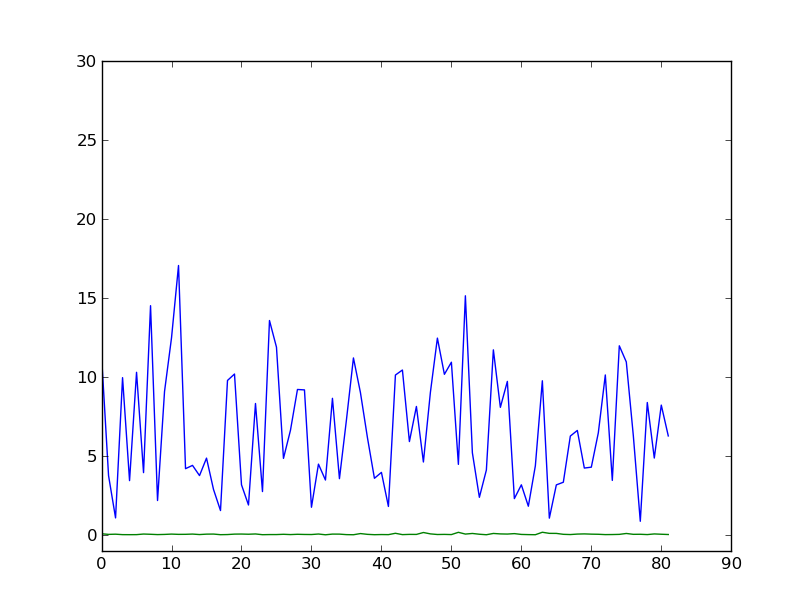
\includegraphics[scale=0.8]{Figures/figure_simulation_consitency.png}
    \rule{35em}{0.5pt}
    \caption[Simulation Consistency]{Variation of fitness function for a PID frequency of 30Hz(Blue) and 100Hz(Green)}
    \label{fig:figure_simulation_consistency}
\end{figure}


    
\section{ Creatures taking advantages of simulation bugs}
Another surprising behaviour in the simulation is the fact that the learning algorithm can take advantage of some of the existing bugs in the simulation. This results was also observed by Karl Sims \cite{karl}. In the simulation when initialising the creature in its starting position, the velocity and position where reinitialised to the starting situation.The problem is that using the approximation of ODE for collision using, some hidden parameters in the simulation were not reinitialised when moving the creature back to its starting position. Therefore, the creature could have some of its blocks under the ground, and was jumping in a really unrealistic way because of this bug. The learning algorithm learned to find the bug and all the best solution were using this bug to jump very far and have a high value for the fitness function.
    
\section { Comparison }

This section present different curves obtained for the different learning method and learning model. In each graph, the we present the evolution of the evaluation of the fitness function which is the distance that a four-legged creature has walked during the learning period.


\begin{figure}[htbp]
    \centering
    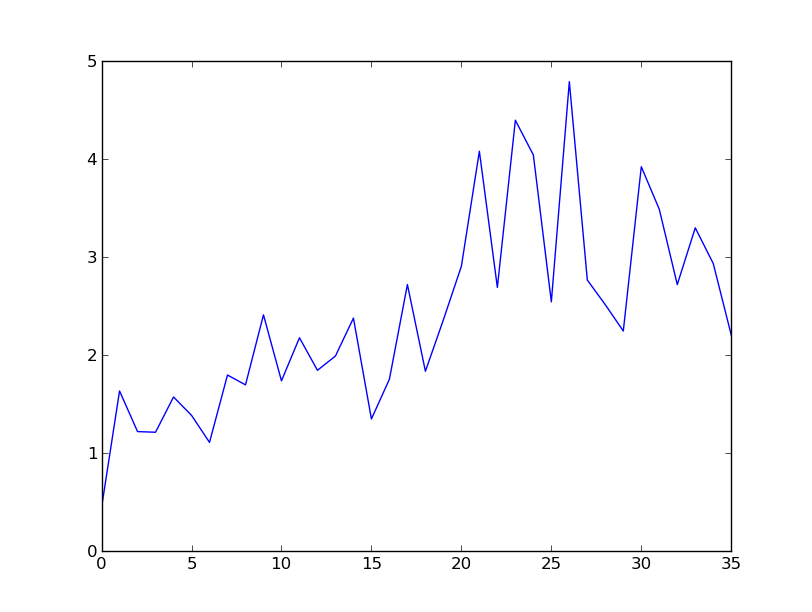
\includegraphics[scale=0.5]{Figures/simplex_fourier.png}
    \rule{35em}{0.5pt}
    \caption[Learning Method : Simplex, Model : Fourier Decomposition]{Learning Method : Simplex, Model : Fourier Decomposition}
    \label{fig:simplex_fourier}
\end{figure}


\begin{figure}[htbp]
    \centering
    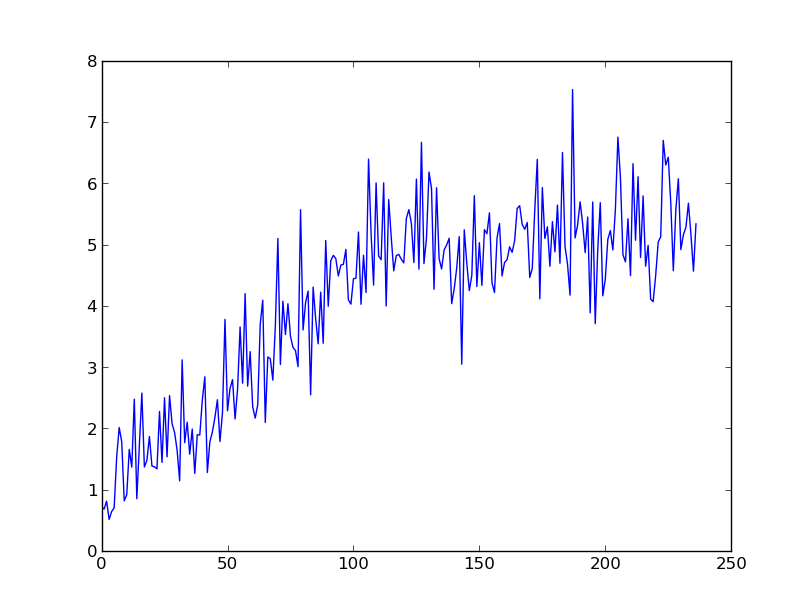
\includegraphics[scale=0.5]{Figures/gen_fourier.png}
    \rule{35em}{0.5pt}
    \caption[Learning Method : GA, Model : Fourier Decomposition]{Learning Method : Genetic Algorithm, Model : Fourier Decomposition}
    \label{fig:simplex_fourier}
\end{figure}

\begin{figure}[htbp]
    \centering
    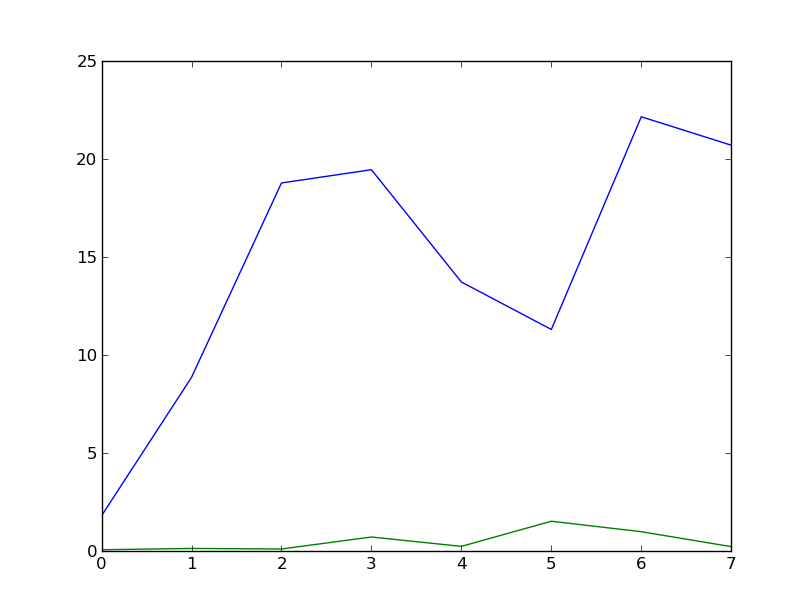
\includegraphics[scale=0.5]{Figures/cpg_simplex.png}
    \rule{35em}{0.5pt}
    \caption[Learning Method : GA, Model : CPG]{Learning Method : Genetic Algorithm, Model : CPG}
    \label{fig:cpg_gen}
\end{figure}


\begin{figure}[htbp]
    \centering
    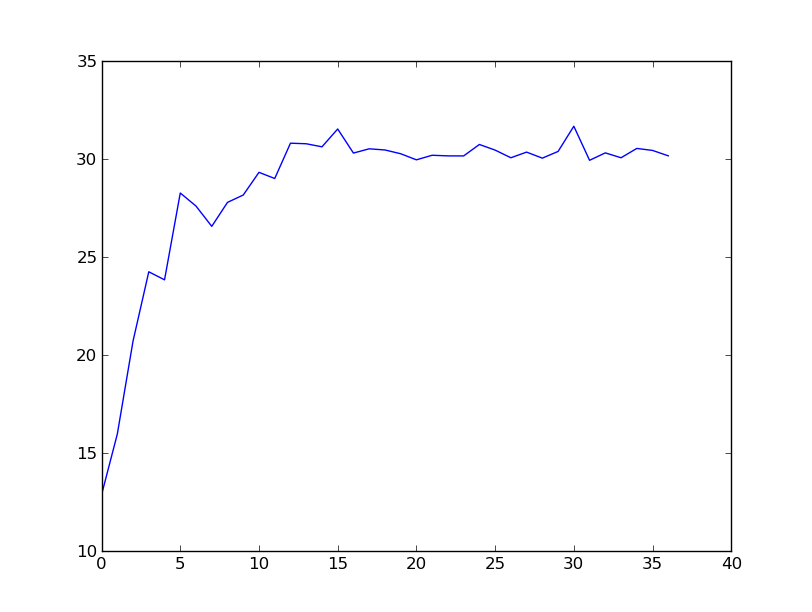
\includegraphics[scale=0.5]{Figures/cpg_gen.png}
    \rule{35em}{0.5pt}
    \caption[Learning Method : GA, Model : CPG]{Learning Method : Genetic Algorithm, Model : CPG}
    \label{fig:cpg_gen}
\end{figure}

\begin{figure}[htbp]
    \centering
    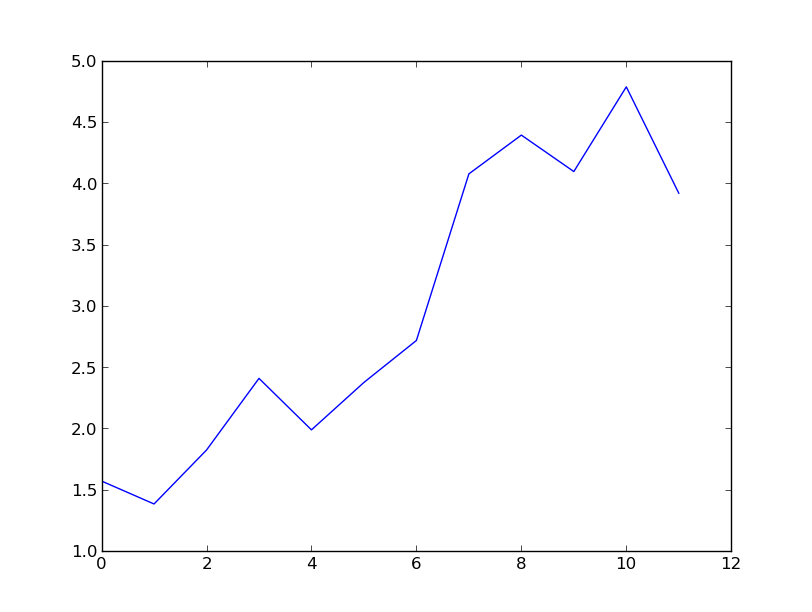
\includegraphics[scale=0.5]{Figures/esn_simplex.png}
    \rule{35em}{0.5pt}
    \caption[Learning Method : Simplex, Model : LMS]{Learning Method : Simplex, Model : Liquid State Machine}
    \label{fig:esn_simplex}
\end{figure}

\begin{figure}[htbp]
    \centering
    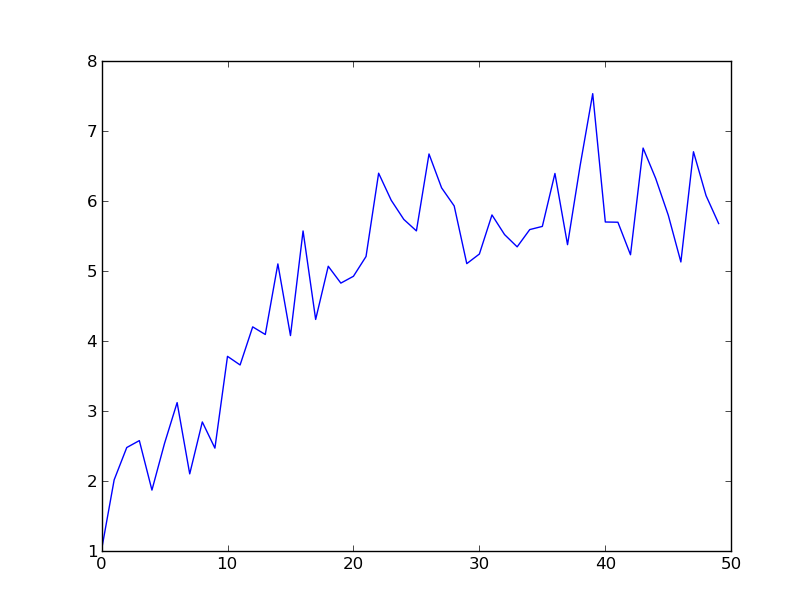
\includegraphics[scale=0.5]{Figures/esn_gen.png}
    \rule{35em}{0.5pt}
    \caption[Learning Method : GA, Model : Liquid State Machine]{Learning Method : Genetic Algorithm, Model : Liquid State Machine}
    \label{fig:esn_gen}
\end{figure}


One of the feature that we can observe in comparing the genetic algorithm and the Nelder Mead method over the different models, is that the genetic algorithm is slower, however it converge towards a higher value. This is an expected behaviour as the simplex is a downhill method and therefore converge towards a local minima. One of the example of the convergence of the Nelder-Mead method towards a local extrema that was encountered was a situation where the creature seems to have learn how to push on one leg only to move. 

The best results have been obtained using the CPG and the Genetic Algorithm (see learning curves). In their architecture, central pattern generator follow the physical shape of the creature, where the Fourier decomposition and the liquid state machine models are independent of it. Therefore, it is easier to train such a model, because it requires less parameters to produce the angles functions. However we could expect to have better results after a long training for the Fourier decomposition and the liquid state machine as well as they are more general models but it is not the case in these results : the learning algorithms are stuck in local minima for these models.



% In the second part of the project, my focus will be on improving the learning algorithms to lead to better solutions. One of the main problem of the movements of these structures is that it optimizes a given paramter (speed, distance with a certain amount of energy, rotation velocity...) but it does not give any control on the structure. In Modular and Swarm Robotics, if we want to make use of such creatures, we need to be able to interact with them, to modify their behaviour. To do so, I want to focus my work on building models to represent how these robots will interact with the world and the orders they receive. Recent deep learning techniques are made possible with the growing accessible computation power and they showed good results on complex problems such as Computer Vision or Sound Recognition. Some of these techniques are good candidate in order to generate complex pattern to understand the structure, generate oscillation for the direct control of joints (Echo State Networks for instance \cite{jaeger2007echo}) and lead to the concept of self-awareness of the mechanical structure of a robot. 

 
% Chapter Template

\chapter{Conclusion} % Main chapter title

\label{} % Change X to a consecutive number; for referencing this chapter elsewhere, use \ref{ChapterX}

\lhead{\emph{Conclusion}} % Change X to a consecutive number; this is for the header on each page - perhaps a shortened title

ADD HERE
 

%\input{Chapters/Chapter3}
%\input{Chapters/Chapter4} 
%\input{Chapters/Chapter5} 
%\input{Chapters/Chapter6} 
%\input{Chapters/Chapter7} 

%----------------------------------------------------------------------------------------
%	THESIS CONTENT - APPENDICES
%----------------------------------------------------------------------------------------

\addtocontents{toc}{\vspace{2em}} % Add a gap in the Contents, for aesthetics

%\appendix % Cue to tell LaTeX that the following 'chapters' are Appendices

% Include the appendices of the thesis as separate files from the Appendices folder
% Uncomment the lines as you write the Appendices

%% Appendix A

\chapter{Appendix Title Here} % Main appendix title

\label{AppendixA} % For referencing this appendix elsewhere, use \ref{AppendixA}

\lhead{Appendix A. \emph{Appendix Title Here}} % This is for the header on each page - perhaps a shortened title

Write your Appendix content here.
%\input{Appendices/AppendixB}
%\input{Appendices/AppendixC}

\addtocontents{toc}{\vspace{2em}} % Add a gap in the Contents, for aesthetics

\backmatter

%----------------------------------------------------------------------------------------
%	BIBLIOGRAPHY
%----------------------------------------------------------------------------------------

\label{Bibliography}

\lhead{\emph{Bibliography}} % Change the page header to say "Bibliography"

\bibliographystyle{unsrtnat} % Use the "unsrtnat" BibTeX style for formatting the Bibliography

\bibliography{Bibliography} % The references (bibliography) information are stored in the file named "Bibliography.bib"

\end{document}
